\documentclass[
  a4paper,
  abstract=true,
  twoside,
  listof=totoc,
  numbers=noenddot,
  bibliography=totoc,
  BCOR1.5cm,
  headsepline,
  DIV12,
  appendixprefix,
  final
] {scrreprt}



% You should select either american or british instead of english here:
\usepackage[ngerman,english]{babel}
\usepackage{fontspec}

% You can choose style "numeric" instead which is common in many papers.
% Without "maxbibnames=99" the bibliography entries only contain "First Name et al."
\usepackage[backend=biber,style=alphabetic,alldates=long,maxbibnames=99]{biblatex}

% FONT SETTINGS & ENCODING
% By default this build setup uses lualatex which supports special characters
% (öäüß<>) out of the box. If you ever want to switch to pdflatex but also
% keep the support for lualatex, add these three packages:
% \usepackage[T1]{fontenc}
% \usepackage[utf8]{luainputenc}
% \usepackage{lmodern}

\usepackage{varioref}           % nice refs
\usepackage{csquotes}
\usepackage{graphicx}           % graphics
\usepackage{caption}            % manipulate fugures
\usepackage{subcaption}         % allow for subfigures
% Also checkout "minted" instead of "listings" - looks much nicer and supports
% more languages but requires "pygmentize" to be available on the command line
\usepackage{listings}           % nice source code listings
\usepackage{xcolor}
\usepackage{booktabs}           % nice tables
\usepackage{microtype}          % better looking text borders
\usepackage{siunitx}            % unified way of setting values with units
\usepackage{array}
\usepackage{fancybox}           % provide nice boxes
\usepackage{fancyvrb}           % algorithm-boxes
\usepackage{pdfpages}
\usepackage{hyphenat}
\usepackage{todonotes}
\usepackage{xspace}
\usepackage{setspace}
\usepackage{fancyhdr}           % enables cool header line and footer line manipulations
\usepackage{lastpage}           % enables the usage of the label "LastPage" to get the
                                % number of pages with \pageref{LastPage}

% use this one last
% (redefines some macros for compatibility with KOMAScript)
\usepackage{scrhack}


\addbibresource{own.bib}

\setcounter{secnumdepth}{3}     % limit enumeration depth
\setcounter{tocdepth}{1}        % limit TOC depth



\definecolor{mygreen}{rgb}{0,0.6,0}
\definecolor{mygray}{rgb}{0.5,0.5,0.5}
\definecolor{mymauve}{rgb}{0.58,0,0.82}

\lstset{ %
  frame=shadowbox,
  rulesepcolor=\color{blue},
  backgroundcolor=\color{white},   % choose the background color; you must add \usepackage{color} or \usepackage{xcolor}
%  basicstyle=\footnotesize,        % the size of the fonts that are used for the code
  breakatwhitespace=false,         % sets if automatic breaks should only happen at whitespace
  breaklines=true,                 % sets automatic line breaking
  captionpos=b,                    % sets the caption-position to bottom
  commentstyle=\color{mygreen},    % comment style
  deletekeywords={...},            % if you want to delete keywords from the given language
  escapeinside={\%*}{*)},          % if you want to add LaTeX within your code
  extendedchars=true,              % lets you use non-ASCII characters; for 8-bits encodings only, does not work with UTF-8
  frame=single,                    % adds a frame around the code
  keepspaces=true,                 % keeps spaces in text, useful for keeping indentation of code (possibly needs columns=flexible)
  keywordstyle=\color{blue},       % keyword style
  language=C,                 % the language of the code
 % morekeywords={*,...},            % if you want to add more keywords to the set
  numbers=left,                    % where to put the line-numbers; possible values are (none, left, right)
  numbersep=7pt,                   % how far the line-numbers are from the code
  numberstyle=\tiny\color{mygray}, % the style that is used for the line-numbers
  rulecolor=\color{black},         % if not set, the frame-color may be changed on line-breaks within not-black text (e.g. comments (green here))
  showspaces=false,                % show spaces everywhere adding particular underscores; it overrides 'showstringspaces'
  showstringspaces=false,          % underline spaces within strings only
  showtabs=false,                  % show tabs within strings adding particular underscores
  stepnumber=1,                    % the step between two line-numbers. If it's 1, each line will be numbered
  stringstyle=\color{mymauve},     % string literal style
  tabsize=2,                       % sets default tabsize to 2 spaces
  title=\lstname                   % show the filename of files included with \lstinputlisting; also try caption instead of title
}

\pagenumbering{Roman}

% remove "pagebackref" for the final version
\usepackage[pdftex,
citebordercolor={0.75 0.75 1},
filebordercolor={0.75 0.75 1},
linkbordercolor={0.75 0.75 1},
% pagebordercolor={0.75 0.75 1},
urlbordercolor={0.75 0.75 1},
pdfborder={0.75 0.75 1},plainpages=false,pdfpagelabels=true]{hyperref}
\hypersetup{%
  pdftitle={Dein Titel},
  pdfauthor={Otto Mustermann},
  pdfkeywords={foo, bar},
}

\tolerance 2414
\hbadness 2414
\emergencystretch 1.5em
\hfuzz 0.3pt
\widowpenalty=10000     % Hurenkinder
\clubpenalty=10000      % Schusterjungen
\vfuzz \hfuzz
\raggedbottom

% use nice footnote indentation
\deffootnote[1em]{1em}{1em}{\textsuperscript{\thefootnotemark}\,}

% some common commands
\newcommand{\drops}{\texorpdfstring{\textsc{Drops}\xspace}{DROPS}}
\newcommand{\LLinux}{\texorpdfstring{L$\!^4$Linux}{L4Linux}}

\newcommand{\NOVA}{NOVA\xspace}
\newcommand{\QEMU}{QEMU\xspace}


% If you know when you will hand in your thesis, enter the date here.
%\date{30. April 2009}
%\newcommand{\printdate}{\@date}

\makeatother
\begin{document}
% use this to generate a list of all todo markers
% \listoftodos{}

\selectlanguage{ngerman}

\begin{singlespace}

    \subject{{\LARGE Diplomarbeit}}

    \title{Dein Titel}

    \author{Otto Mustermann}

    \publishers{Technische Universität Dresden\\
    Fakultät Informatik\\
    Institut für Systemarchitektur\\
    Professur für Betriebssysteme\\
        \begin{minipage}{\textwidth}%\\
            \vspace{6cm}
                {\normalsize }\begin{tabular}{ll}
                                  Betreuender Hochschullehrer: &
                                  Prof.\ Dr.-Ing.\ Horst Schirmeier\tabularnewline
                                  Betreuender Mitarbeiter: &
                                  Dipl.-Inf.\ Dein Betreuer\tabularnewline
            \end{tabular} {\normalsize }
        \end{minipage}}

    \maketitle
\end{singlespace}

\cleardoublepage



\includepdf{images/diplom-aufgabe.pdf}
\cleardoublepage

\selectlanguage{ngerman}

\section*{\vfill{} \thispagestyle{empty}
Selbstständigkeitserklärung}
%\section*{\vfill{} \thispagestyle{empty}
%Statement of authorship}

Hiermit erkläre ich, dass ich diese Arbeit selbstständig verfasst
und keine anderen als die angegebenen Quellen und Hilfsmittel benutzt habe.
%I hereby certify that I have completed this work on my own and without the
%help of anything other than the indicated sources and resources.
\bigskip{}

% CAUTION: In the Nix build, \today likely falls back to 1.1.1980.
\noindent Dresden, den \today % \printdate % if you defined date earlier
\vspace{2.5cm}

\noindent Otto Mustermann \cleardoublepage{}


% NOTE: if you selected british or american above, change that here too
\selectlanguage{english}

\begin{abstract}
% -*- Mode: Latex -*-

%  Zusammenfassung

% Zu einer runden Arbeit gehört auch eine Zusammenfassung, die
% eigenständig einen kurzen Abriß der Arbeit gibt. Eine halbe bis ganze
% DINA4 Seite ist angemessen. Dafür läßt sich keine Gebrauchsanweisung
% geben (für irgendetwas müssen die Betreuer ja auch noch da
% sein).

\ldots abstract \ldots

%%% Local Variables:
%%% TeX-master: "diplom"
%%% End:



\end{abstract}

\cleardoublepage

\tableofcontents{}

\listoftables
\listoffigures

\newpage
% \begin{center}
%   This page is intentionally left blank.
% \end{center}
% Force LaTeX to really emit an empty page.
\vspace*{1em}
\cleardoublepage

%\doublespacing
\chapter{Introduction}
\label{sec:intro}

% Die Einleitung schreibt man zuletzt, wenn die Arbeit im Großen und
% Ganzen schon fertig ist. (Wenn man mit der Einleitung beginnt - ein
% häufiger Fehler - braucht man viel länger und wirft sie später doch
% wieder weg). Sie hat als wesentliche Aufgabe, den Kontext für die
% unterschiedlichen Klassen von Lesern herzustellen. Man muß hier die
% Leser für sich gewinnen. Das Problem, mit dem sich die Arbeit befaßt,
% sollte am Ende wenigsten in Grundzügen klar sein und dem Leser
% interessant erscheinen. Das Kapitel schließt mit einer Übersicht über
% den Rest der Arbeit. Meist braucht man mindestens 4 Seiten dafür, mehr
% als 10 Seiten liest keiner.

\todo{adopt title page}

\todo{adopt disclaimer}

\todo{write introduction}

\section{A Section}

Referencing other chapters: \ref{sec:state} \ref{sec:design}
\ref{sec:implementation} \ref{sec:evaluation} \ref{sec:futurework}
\ref{sec:conclusion}

\begin{table}[htp]
    \centering
    \begin{tabular}{lrr}
        \textbf{Name}      & \textbf{Y} & \textbf{Z}         \\
        \hline
        \textit{Foo}       & 20,614     & \SI{23}{\percent}  \\
        \textit{Bar}       & 9,914      & \SI{11}{\percent}  \\
        \textit{Foo + Bar} & 30,528     & \SI{34}{\percent}  \\
        \hline
        \textit{total}     & 88,215     & \SI{100}{\percent} \\

    \end{tabular}
    \caption[Some interesting numbers]{Various very important looking numbers and sums.}
    \label{tab:numbers}
\end{table}

More text referencing Table~\ref{tab:numbers}.

\section{Another Section}

\begin{figure}[tbp]
    \centering
    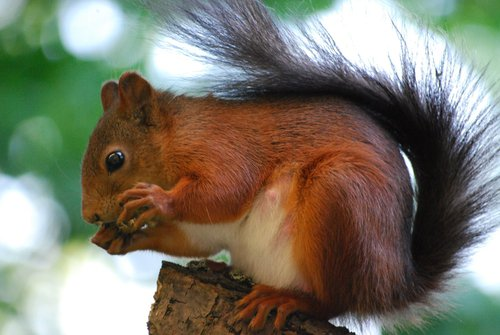
\includegraphics[width=0.8\textwidth]{images/squirrel}
    \caption[Short description]{A long description of this squirrel figure.
    Image taken from
    \url{http://commons.wikimedia.org/wiki/File:Sciurus-vulgaris_hernandeangelis_stockholm_2008-06-04.jpg}}
    \label{fig:squirrel}
\end{figure}

Citing \cite{bellard2005qfa} other documents \cite{bellard2005qfa, boileau06}
and Figure~\ref{fig:squirrel}.

Something with umlauts and a year/month date:
\cite{becher04:_feurig_hacken_mit_firew}.

And some online resources: \cite{green04}, \cite{patent:4819234}


\section{Yet Another Section}

\todo{add content}

\begin{figure}[tbp]
    \missingfigure{Come up with a mindblowing figure.}
    \caption{A mindblowing figure}
    \label{fig:todo}
\end{figure}

\section{Test commands}

\drops \LLinux \NOVA \QEMU
\texttt{memcpy}
A sentence about BASIC. And a correctly formatted one about ECC\@.

\cleardoublepage

%%% Local Variables:
%%% TeX-master: "diplom"
%%% End:

\chapter{Technical Background}
\label{sec:state}

% Hier werden zwei wesentliche Aufgaben erledigt:

% 1. Der Leser muß alles beigebracht bekommen, was er zum Verständnis
% der späteren Kapitel braucht. Insbesondere sind in unserem Fach die
% Systemvoraussetzungen zu klären, die man später benutzt. Zulässig ist
% auch, daß man hier auf Tutorials oder Ähnliches verweist, die hier auf
% dem Netz zugänglich sind.

% 2. Es muß klar werden, was anderswo zu diesem Problem gearbeitet
% wird. Insbesondere sollen natürlich die Lücken der anderen klar
% werden. Warum ist die eigene Arbeit, der eigene Ansatz wichtig, um
% hier den Stand der Technik weiterzubringen? Dieses Kapitel wird von
% vielen Lesern übergangen (nicht aber vom Gutachter ;-), auch später
% bei Veröffentlichungen ist "Related Work" eine wichtige Sache.

% Viele Leser stellen dann später fest, daß sie einige der Grundlagen
% doch brauchen und blättern zurück. Deshalb ist es gut,
% Rückwärtsverweise in späteren Kapiteln zu haben, und zwar so, daß man
% die Abschnitte, auf die verwiesen wird, auch für sich lesen
% kann. Diese Kapitel kann relativ lang werden, je größer der Kontext
% der Arbeit, desto länger. Es lohnt sich auch! Den Text kann man unter
% Umständen wiederverwenden, indem man ihn als "Tutorial" zu einem
% Gebiet auch dem Netz zugänglich macht.

% Dadurch gewinnt man manchmal wertvolle Hinweise von Kollegen. Dieses
% Kapitel wird in der Regel zuerst geschrieben und ist das Einfachste
% (oder das Schwerste weil erste).

\ldots state of the art \ldots

\todo{write state}

\cleardoublepage

%%% Local Variables:
%%% TeX-master: "diplom"
%%% End:

\chapter{Design}
\label{sec:design}

% Ist das zentrale Kapitel der Arbeit. Hier werden das Ziel sowie die
% eigenen Ideen, Wertungen, Entwurfsentscheidungen vorgebracht. Es kann
% sich lohnen, verschiedene Möglichkeiten durchzuspielen und dann
% explizit zu begründen, warum man sich für eine bestimmte entschieden
% hat. Dieses Kapitel sollte - zumindest in Stichworten - schon bei den
% ersten Festlegungen eines Entwurfs skizziert werden.
% Es wird sich aber in einer normal verlaufenden
% Arbeit dauernd etwas daran ändern. Das Kapitel darf nicht zu
% detailliert werden, sonst langweilt sich der Leser. Es ist sehr
% wichtig, das richtige Abstraktionsniveau zu finden. Beim Verfassen
% sollte man auf die Wiederverwendbarkeit des Textes achten.

% Plant man eine Veröffentlichung aus der Arbeit zu machen, können von
% diesem Kapitel Teile genommen werden. Das Kapitel wird in der Regel
% wohl mindestens 8 Seiten haben, mehr als 20 können ein Hinweis darauf
% sein, daß das Abstraktionsniveau verfehlt wurde.

\ldots design \ldots

\todo{write design}

\cleardoublepage

%%% Local Variables:
%%% TeX-master: "diplom"
%%% End:

\chapter{Implementation}
\label{sec:implementation}

% Hier greift man einige wenige, interessante Gesichtspunkte der
% Implementierung heraus. Das Kapitel darf nicht mit Dokumentation oder
% gar Programmkommentaren verwechselt werden. Es kann vorkommen, daß
% sehr viele Gesichtspunkte aufgegriffen werden müssen, ist aber nicht
% sehr häufig. Zweck dieses Kapitels ist einerseits, glaubhaft zu
% machen, daß man es bei der Arbeit nicht mit einem "Papiertiger"
% sondern einem real existierenden System zu tun hat. Es ist sicherlich
% auch ein sehr wichtiger Text für jemanden, der die Arbeit später
% fortsetzt. Der dritte Gesichtspunkt dabei ist, einem Leser einen etwas
% tieferen Einblick in die Technik zu geben, mit der man sich hier
% beschäftigt. Schöne Bespiele sind "War Stories", also Dinge mit denen
% man besonders zu kämpfen hatte, oder eine konkrete, beispielhafte
% Verfeinerung einer der in Kapitel 3 vorgestellten Ideen. Auch hier
% gilt, mehr als 20 Seiten liest keiner, aber das ist hierbei nicht so
% schlimm, weil man die Lektüre ja einfach abbrechen kann, ohne den
% Faden zu verlieren. Vollständige Quellprogramme haben in einer Arbeit
% nichts zu suchen, auch nicht im Anhang, sondern gehören auf Rechner,
% auf denen man sie sich ansehen kann.

\ldots implementation \ldots

\cleardoublepage

%%% Local Variables:
%%% TeX-master: "diplom"
%%% End:

\chapter{Evaluation}
\label{sec:evaluation}

% Zu jeder Arbeit in unserem Bereich gehört eine Leistungsbewertung. Aus
% diesem Kapitel sollte hervorgehen, welche Methoden angewandt worden,
% die Leistungsfähigkeit zu bewerten und welche Ergabnisse dabei erzielt
% wurden. Wichtig ist es, dem Leser nicht nur ein paar Zahlen
% hinzustellen, sondern auch eine Diskussion der Ergebnisse
% vorzunehmen. Es wird empfohlen zunächst die eigenen Erwartungen
% bezüglich der Ergebnisse zu erläutern und anschließend eventuell
% festgestellte Abweichungen zu erklären.

\ldots evaluation \ldots

\todo{write evaluation}

\cleardoublepage

%%% Local Variables:
%%% TeX-master: "diplom"
%%% End:

\chapter{Future Work}
\label{sec:futurework}

\ldots future work \ldots

\cleardoublepage

%%% Local Variables:
%%% TeX-master: "diplom"
%%% End:

\chapter{Conclusion And Outlook}
\label{sec:conclusion}

%  Schlußfolgerungen, Fragen, Ausblicke

% Dieses Kapitel ist sicherlich das am Schwierigsten zu schreibende. Es
% dient einer gerafften Zusammenfassung dessen, was man gelernt hat. Es
% ist möglicherweise gespickt von Rückwärtsverweisen in den Text, um dem
% faulen aber interessierten Leser (der Regelfall) doch noch einmal die
% Chance zu geben, sich etwas fundierter weiterzubilden. Manche guten
% Arbeiten werfen mehr Probleme auf als sie lösen. Dies darf man ruhig
% zugeben und diskutieren. Man kann gegebenenfalls auch schreiben, was
% man in dieser Sache noch zu tun gedenkt oder den Nachfolgern ein paar
% Tips geben. Aber man sollte nicht um jeden Preis Fragen, die gar nicht
% da sind, mit Gewalt aufbringen und dem Leser suggerieren, wie
% weitsichtig man doch ist. Dieses Kapitel muß kurz sein, damit es
% gelesen wird.

\ldots conclusion \ldots

\cleardoublepage

%%% Local Variables:
%%% TeX-master: "diplom"
%%% End:


\appendix

%\addchap{Glossar}

% makeglossaries diplom
%\printglossary[style=altlist]
%\printglossary[type=\acronymtype,style=long]

\printbibliography
\iffalse
    % an aid for Kile autocompletion
    \bibliography{own.bib}
\fi

\end{document}
